\section{Project Management}
Due to this project being spread over almost an entire year, a certain amount of management needs to be maintained in order to ensure that work does not fall behind.

\subsection{Gannt Chart}
One method used in this project to keep track of progress is a Gannt Chart.
This is a way of showing what work should be being done when, and allowing tasks which overrun to be easily noticed.
\\
\begin{sidewaysfigure}
	\centering
	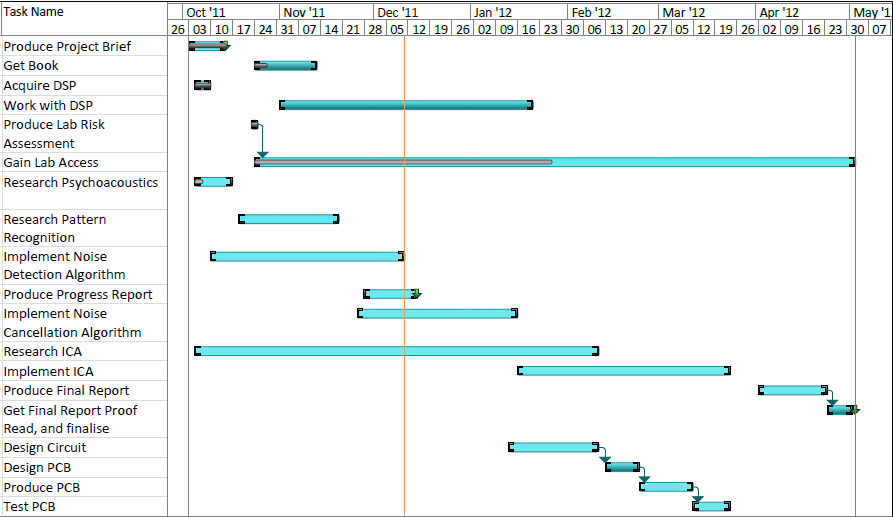
\includegraphics[width=\textwidth]{./img/ganntori.png}
	\caption{The Gannt chart for this project as originally produced}
	\label{fig:gannt}
\end{sidewaysfigure}

\noindent
The Gannt chart shown in figure~\ref{fig:gannt} changes regularly as time gets reallocated and tasks get completed ahead or behind schedule.
As of the time of writing the progress report the gannt chart stood as shown in figure ~\ref{fig:newgannt}.
By the end of the project it had changed further still, and could be seen as
\\
\begin{sidewaysfigure}
	\centering
	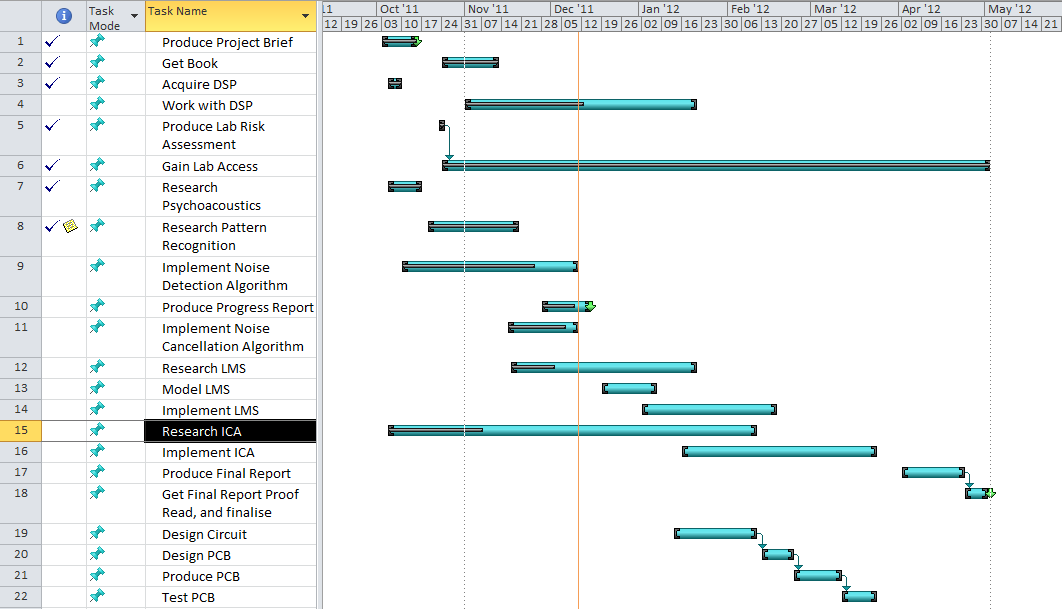
\includegraphics[width=\textwidth]{./img/ganntnew.png}
	\caption{The Gannt chart for this project as of the progress report}
	\label{fig:newgannt}
\end{sidewaysfigure}

\noindent
A few differences can be seen between these two charts.
The majority of the differences are tasks that have been achieved, however the most significant difference is the introduction of the sections on LMS which will be discussed in section~\ref{sec:LMS}.
\\
\\
Futher changes can be seen between this one and the gannt chart of how the events actually panned out.
In this later gannt chart a larger emphasis was placed on the production of a PCB to run the algorithm.

\subsection{Weekly Tracker}
While Gannt Charts clearly show what should be being done and when, they are less representative of what should be being achieved in the short term.
As such the `Weekly Tracker' was developed in order to show what tasks needed to be achieved in the week, and to follow whether the project was on track on a weekly basis.
\\
\\
This is a sheet containing a list of tasks to be worked on during the coming week, including a review date on which the progress of each of these tasks would be noted and compared against the required progress.
\\
\\
Each task has a task name; also each task has space for notes at the beginning and end of the week.
Along with this, each task has a rank from 0 to 10 for minimum acceptable completion.
This is essentially the minimum percentage of the task that required to have been completed by the end of the week to remain on track.
Using a rank below 10 here allows for tasks to span multiple weeks, by increasing the required rank while progressing through the project.
There is also a rank for task completion.
This rank is out of the entire task, not just the amount required for the week, allowing progress beyond that expected for that week to be noted.
In the event of progression beyond the scope required by the overall task, this would be ranked as `+'.
At the end of the week on the review date, the sum of the differences between required and completed ranks would give a score for the week.
A negative score would denote that the project is behind schedule, whereas a positive score denotes that it is ahead of schedule.
A score of 0 indicating that it is on schedule.
An example of these can be seen in appendix \ref{appendix:weeklytracker}.
\\
\\
Table \ref{tab:scorings} shows the scores achieved on these weekly trackers.
\begin{table}[H]
	\centering
	\begin{tabular}[c]{| c | l | l | c |}
		\hline
		Sheet	& Start	& End	& Score \\
		\hline
		1	& 05/10/2011	& 09/10/2011	& -6	\\
		2	& 10/10/2011	& 16/10/2011	& -2	\\
		3	& 16/10/2011	& 23/10/2011	& -1	\\
		4	& 23/10/2011	& 30/10/2011	& -5	\\
		5	& 01/11/2011	& 06/11/2011	& -10	\\
		6	& 09/11/2011	& 13/11/2011	& -2	\\
		7	& 13/11/2011	& 20/11/2011	& -12	\\
		8	& 21/11/2011	& 27/11/2011	& -6	\\
		9	& 27/11/2011	& 04/12/2011	& -6	\\
		10	& 04/12/2011	& 11/12/2011	& 0	\\
		11	& 11/12/2011	& 18/12/2011	& -1	\\
		12	& 18/12/2011	& 08/01/2012	& -7	\\
		13	& 08/01/2012	& 29/01/2012	& -7	\\
		14	& 29/01/2012	& 05/02/2012	& -3	\\
		15	& 05/02/2012	& 12/02/2012	& 0	\\
		16	& 12/02/2012	& 19/02/2012	& -1	\\
		17	& 19/02/2012	& 26/02/2012	& -3	\\
		18	& 26/02/2012	& 04/03/2012	& 7	\\
		19	& 26/02/2012	& 04/03/2012	& 7	\\
		20	& 04/03/2012	& 11/03/2012	& -5	\\
		21	& 11/03/2012	& 18/03/2012	& -10	\\
		22	& 18/03/2012	& 01/04/2012	& -7	\\
		23	& 01/04/2012	& 15/04/2012	& -5	\\
		24	& 15/04/2012	& 22/04/2012	& 	\\
		\hline
	\end{tabular}
	\caption{Scorings of the weekly tracker}
	\label{tab:scorings}
\end{table}

\noindent These scorings show that the project was consistently behind schedule.
This was largely due to not fully anticipating how long certain aspects of the project would take, and unforeseen external factors.
Also the design of the weekly tracker doesn't particularly allow for scoring ahead of schedule.
This is because when work is completed significantly beyond the scope of the task an additional score of only 1 can be achieved, whereas negative scores are easier to achieve.


\subsection{Milestones}
In order to determine the state of the system, a collection of milestones has been set.
At each one the system would be able to demonstrate a level of functionality.
This would allow any major progress in the system to be noted and would allow the progress of the system to be observed.
Each milestone has a list of requirements which have to be met before it can be classed as achieved.
These milestones do not have to be met in the order stated, and some of them will be worked on in parallel, though in most cases the milestones build on the previous ones.

\begin{table}[H]
	\centering
	\begin{tabular}[c]{| c | l | c |}
		\hline
		No.	& Milestone		& Achieved? \\
		\hline
		1	& Record/replay audio	& X \\
		2	& Cancellation algorithm & X \\
		3	& Cancellation on DSP	& X \\
		4	& Create PCB		& \\
		5	& LMS algorithm		& \\
		6	& LMS on DSP		& \\
		7	& Add ICA		& \\
		\hline
	\end{tabular}
	\caption{The milestones set for the project}
	\label{tab:milestones}
\end{table}
